% !TeX spellcheck = en_US
\section{Contract Law}
\subsection{Definition contract}
A contract determines:
\begin{compactitem}
	\item Who
	\item What
	\item Where
	\item How
	\item When
	\item For how long
	\item For how much
\end{compactitem}
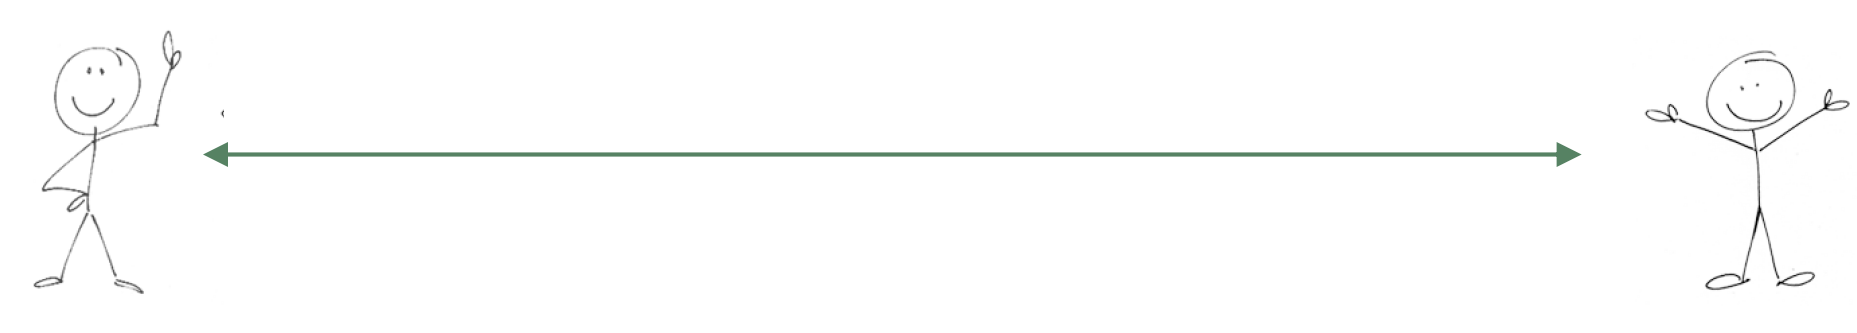
\includegraphics[width=1\linewidth]{images/contract1}
\begin{compactitem}
	\item Freedom of contract: freedom to chose a contracting party and the content / the conditions
	\item Offer and acceptance
	\item Two or more parties
	\item Mutual consent over «essentialia negotii» (essential terms)
	\item As a rule: No written form!
\end{compactitem}
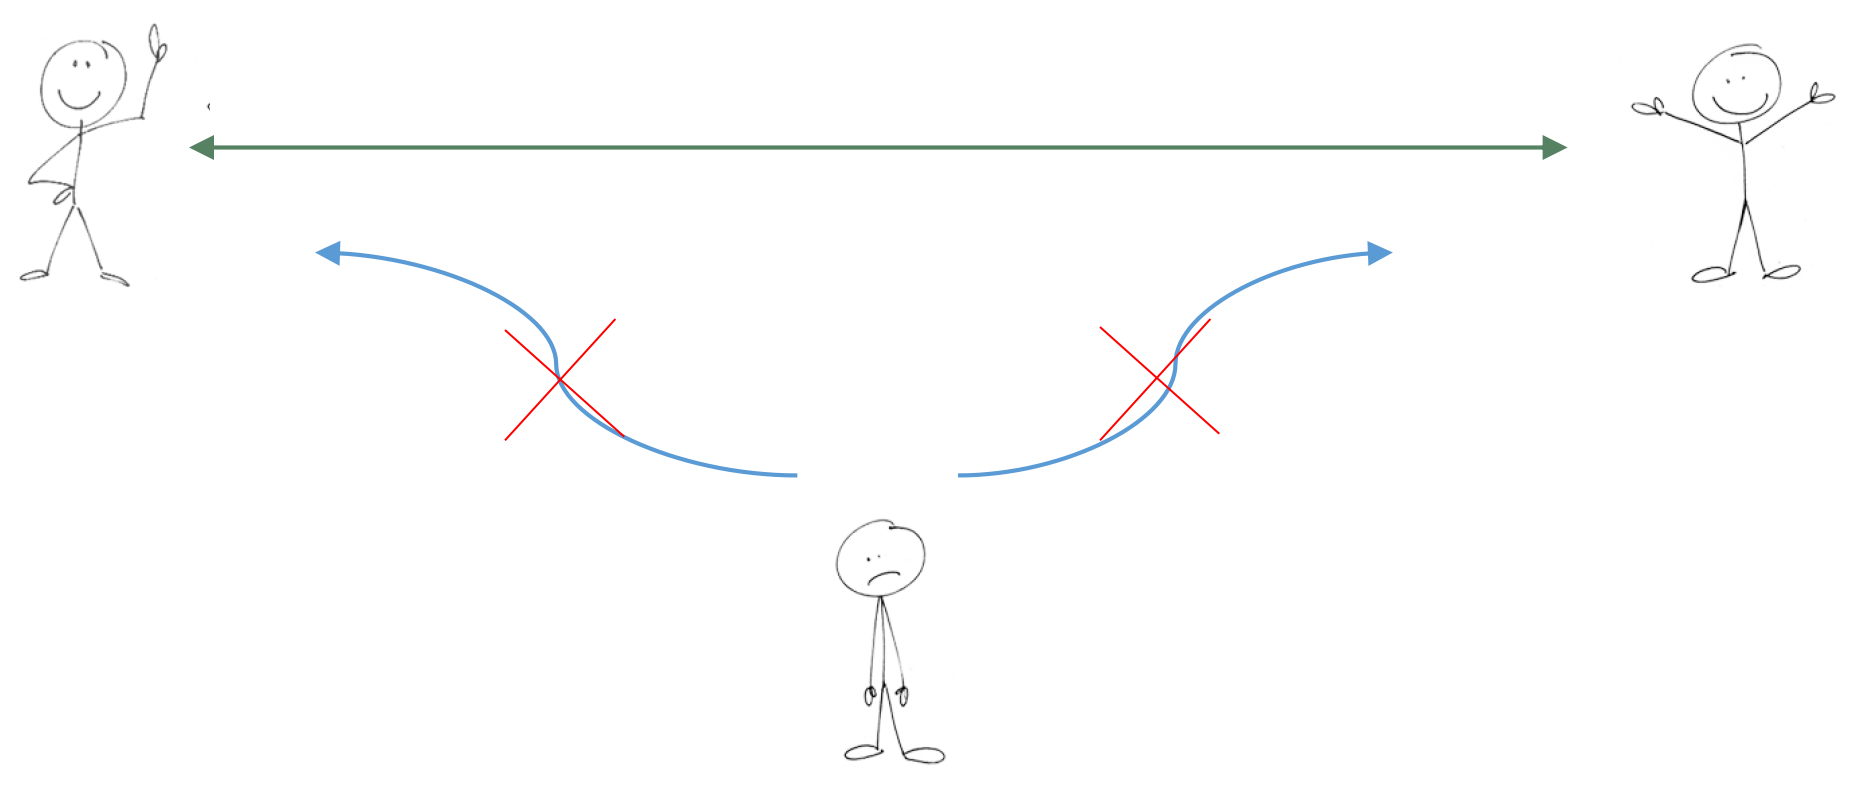
\includegraphics[width=1\linewidth]{images/contract2}
\begin{compactitem}
	\item Legal impact: only in relation to the contracting party
	\item Contract creates rights and obligations between the parties
	\item Any change to the contract must be mutually agreed
	\item Enforcement only against the contracting party
\end{compactitem}

\subsection{Freedom of contract}
\begin{compactitem}
	\item \textbf{Freedom to conclude or not conclude a contract, freedom to terminate:} No one is obliged to conclude a contract. Exemptions: A legal provision to conclude a contract is the obligation of every car owner to effect an insurance.
	\item \textbf{Freedom to choose the contractual partner:} Everyone has the right to choose his/her contractual partner. Exceptions: minors cannot validly conclude certain (majority!) contracts.
	\item \textbf{Freedom to establish the contracts content:} If the content is forbidden by law the contract is null and void. Swiss law, in particular the Swiss Code of Obligations, contains few mandatory provisions that need to be taken into account.
\end{compactitem}

\subsection{Form}
\begin{compactitem}
	\item As a rule: No written form!
	\item A contract may be concluded orally or even without using words but by a consenting behavior (tacit)
	\item Written form is prescribed only if one or both parties require(s) protection (examples: apprenticeship contract, inheritance contracts, real estate contracts)
	\item Most parties choose the written form voluntarily in order to have clarity and	proof
	\item What is written form? -> personal signature (Art. 13 ff. of OR)
	\item Digital signature does not meet this requirement, it merely authenticates the	individual!
\end{compactitem}

\subsection{Swiss code of obligations}
\textbf{General provisions on conclusion of contracts performance and non-performance:}
\begin{compactenum}
	\item Conclusion of the contract ( How to reach consent: mutual expression of intent)
	\item Form of contracts
	\item Defects in consent: error, fraud, duress
	\item Representation: authorization to act on someone else’s behalf
	\item Performance of obligations ( place, time, payment )
	\item Breach of contract: the consequences of non-performance of obligations
	\item Third parties
	\item Time limits
	\item Special types of contracts
\end{compactenum}
\textbf{Types of contracts codified:}
\begin{compactitem}
	\item Sale and Exchange
	\item Lease
	\item Loan
	\item Employment Contract
	\item Contract for Work and Services
	\item Services Contract
	\item Commission
	\item Guarantee
\end{compactitem}

\subsection{Types of contracts}
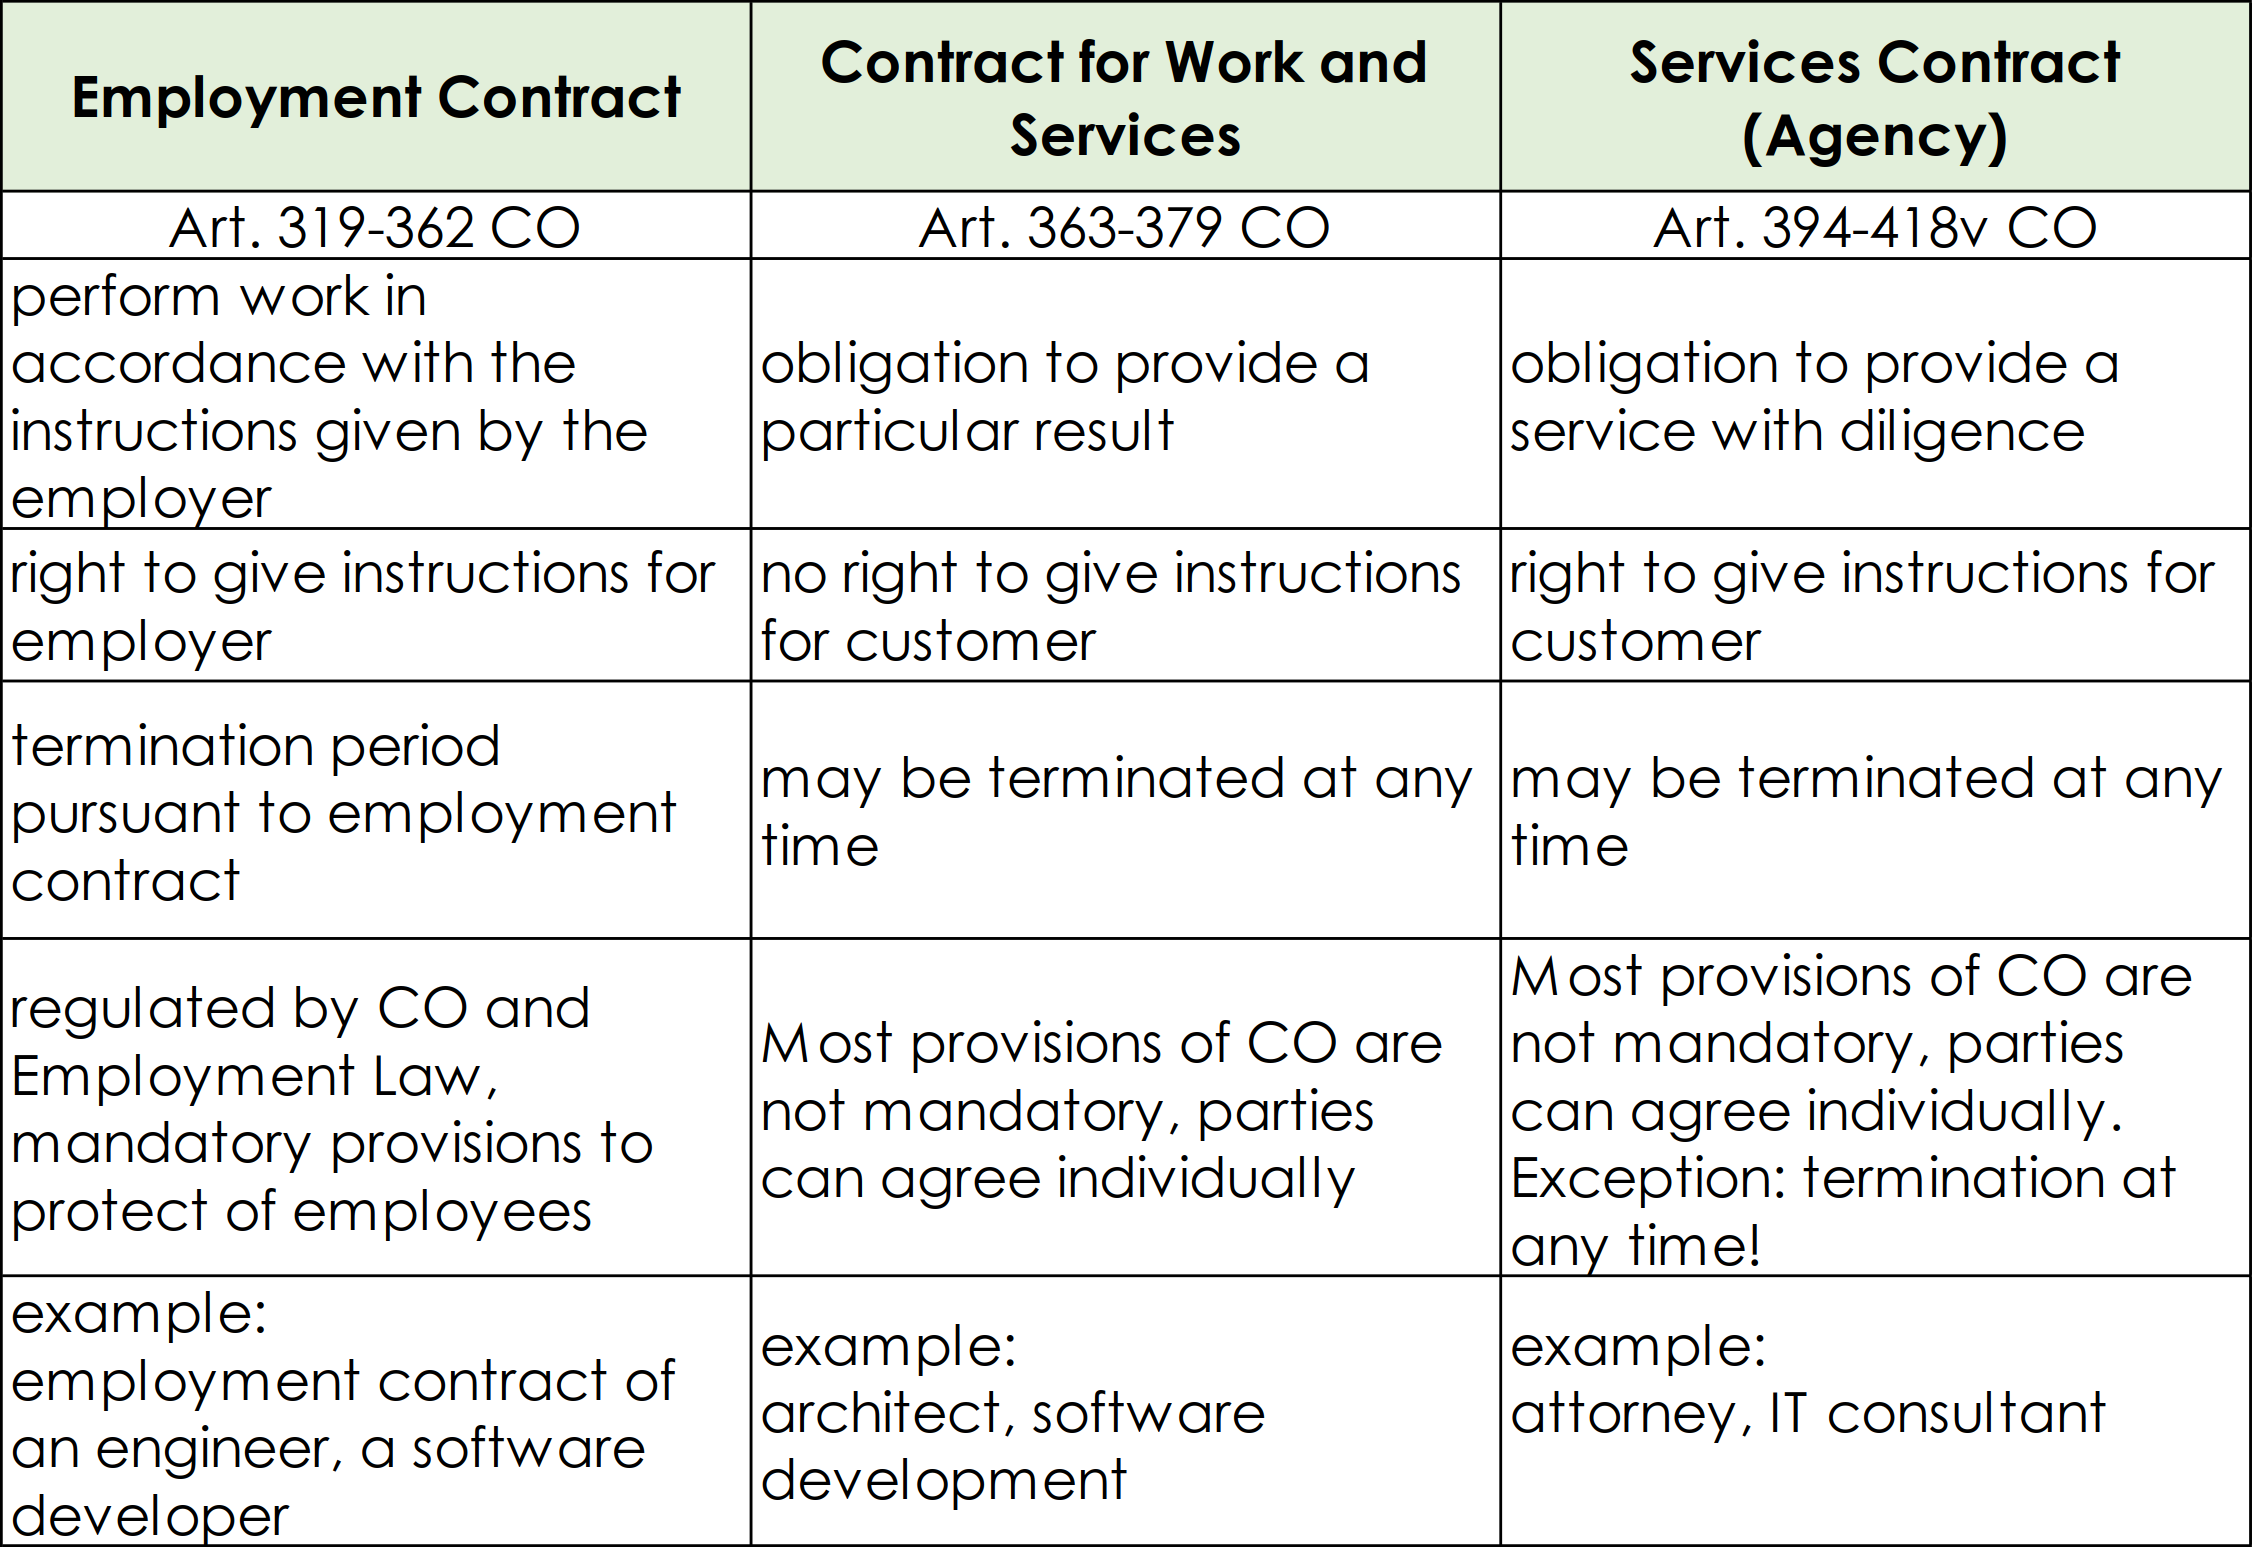
\includegraphics[width=1\linewidth]{images/typesofcontract}

\subsection{Contract for work and services}
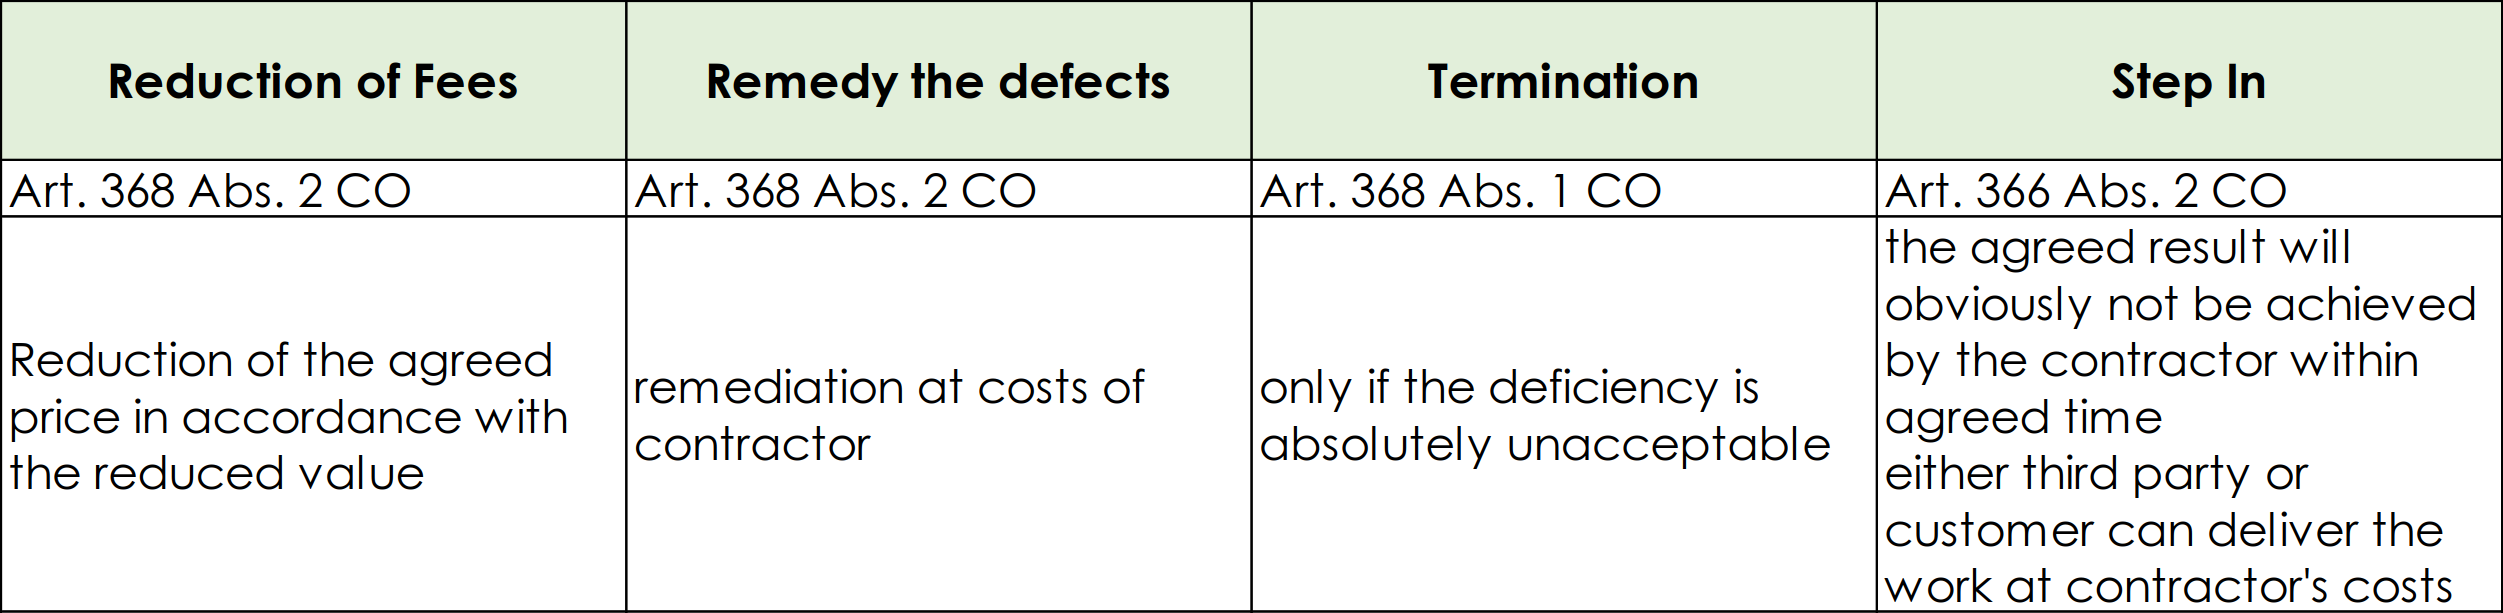
\includegraphics[width=1\linewidth]{images/contractforwork}

\subsection{General terms and conditions}
General Terms and Conditions are predefined contracts a provider/seller concludes with its customers. \\
\textbf{Aim of General Terms and Conditions:}
\begin{compactitem}
	\item Gain efficiency
	\item Allocate risk («NO WARRANTIES NO LIABILITIES»)
	\item Terms and Conditions for sale in webshops, licenses for software etc. apply once the box is ticked, whether or not you have read them!
\end{compactitem}
\textbf{When do they apply?}\\
General Terms and Conditions of a provider / seller only apply if the customer has accepted them. The provider/seller is obliged to bring the GTCs to the attention of the customer (explicit reference) prior to the conclusion of the individual contract/provision of goods or services. General Terms and Conditions provided after acceptance by customer are not valid and do not apply.\\
\textbf{Limitations:}
\begin{compactitem}
	\item \textbf{Rule of «Unusualness»:} If the General Terms and Conditions contain provisions the consumer could	not have expected, such provisions are interpreted to the disadvantage of the provider/seller.
	\item \textbf{Rule of «Unclarity»:}	If the General Terms and Conditions contain provisions that are unclear to the consumer, such provisions are interpreted to the disadvantage of the provider/seller.
	\item \textbf{Unfair competition:} Pursuant to Art. 8 of the Federal Act against Unfair Competition (UCA), General Terms and Conditions are deemed unfair if, in violation of good faith, they create a considerable and unjustified disparity between the vendor and the customer.
\end{compactitem}

\subsection{Framework Agreements}
Framework agreements set the frame for larger projects and contain general terms. The what when how is then determined in detail in Work Orders.
\begin{compactenum}
	\item Assistance and collaboration duties
	\item Contract term
	\item Liability
	\item Costs
	\item Security standards and technical standards
	\item Data protection and confidentiality
	\item Conflict prevention and conflict management
	\item Applicable law and jurisdiction
\end{compactenum}

\subsection{The Consequences of Non-Performance of Obligations}
Prerequisites for liability pursuant to art. 97 CO and burden of proof:
\begin{compactitem}
	\item damage (amount)
	\item breach of a contract
	\item causality between the damage and the breach
	\item misconduct attributable to the obligor (assumed)
\end{compactitem}
\textbf{Penalties:}\\
The contractual penalty must be contractually agreed and is due in the event of an infringement of a contractual duty, such as:
\begin{compactitem}
	\item Non-performance
	\item Inadequate performance
	\item Delay
	\item Confidentiality
	\item Non-competition clause
	\item Data Protection / Security
\end{compactitem}
Contractual penalties are due even if the other contracting party has not incurred a damage. If a damage has occurred, damages are to be paid if the damages exceed the amount of the contractual penalty. The parties may agree in the contract that contractual penalties are due in addition to damages. If the amount of the contractual penalty is extremely high, a court may reduce them.

\subsection{Obligations in tort (Delikt)}
No contract, but a party is held liable for damages!
\begin{compactitem}
	\item Liability of persons lacking capacity to consent (Art. 54 OR)
	\item Liability of employers (Art. 55 OR)
	\item Liability for animals (Art. 56 OR)
	\item Liability of property owners (Art. 58 OR)
	\item Liability in respect of electronic signatures (Art. 59a OR)
	\item Liability of civil servants and public officials (Art. 61 OR)
\end{compactitem}
Prerequisites for liability pursuant (Haftung) to Art. 41 OR and burden of proof:
\begin{compactitem}
	\item damage (amount)
	\item illegality
	\item causality between the damage and the breach
	\item misconduct attributable to the defendant
\end{compactitem}

\subsection{Time limits}
\textbf{Contract Law:}\\
After ten years unless otherwise provided by federal civil law (Art. 127 OR).\\
\textbf{Obligations in tart:}\\
One year from the date on which the injured party became aware of the loss/damage and of the identity of the person liable; in any event ten years after the date on which the loss/damage was caused (Art. 60 OR).

\subsection{Legal base}
\subsubsection{Consensus - ART. 1 OR}
\begin{compactenum}
	\item The conclusion of a contract requires a mutual expression of intent by the parties.
	\item The expression of intent may be express or implied.
\end{compactenum}

\textit{\begin{compactenum}
	\item Zum Abschlusse eines Vertrages ist die übereinstimmende gegenseitige Willensäusserung der Parteien erforderlich.
	\item Sie kann eine ausdrückliche oder stillschweigende sein.
\end{compactenum}}

\subsubsection{Freedom of contract - ART. 19 OR}
\begin{compactenum}
	\item The terms of a contract may be freely determined within the limits of the law.
	\item Clauses that deviate from those prescribed by law are admissible only	where the law does not prescribe mandatory forms of wording or where deviation from the legally prescribed terms would \textbf{contravene public policy, morality or rights of personal privacy}.
\end{compactenum}

\textit{\begin{compactenum}
	\item Der Inhalt des Vertrages kann innerhalb der Schranken des Gesetzes beliebig festgestellt werden.
	\item Von den gesetzlichen Vorschriften abweichende Vereinbarungen sind nur zulässig, wo das Gesetz nicht eine unabänderliche Vorschrift aufstellt oder die Abweichung nicht einen Verstoss gegen die öffentliche Ordnung, gegen die guten Sitten oder gegen das Recht der Persönlichkeit in sich schliesst.
\end{compactenum}}

\subsubsection{Freedom of contract - ART. 20 OR}
\begin{compactenum}
	\item A contract is \textbf{void} if its terms are \textbf{impossible, unlawful or immoral}.
	\item However, where the defect pertains only to certain terms of a contract, those terms alone are void unless there is cause to assume that the contract would not have been concluded without them.
\end{compactenum}

\textit{\begin{compactenum}
	\item Ein Vertrag, der einen unmöglichen oder widerrechtlichen Inhalt hat oder gegen die guten Sitten verstösst, ist nichtig.
	\item Betrifft aber der Mangel bloss einzelne Teile des Vertrages, so sind nur diese nichtig, sobald nicht anzunehmen ist, dass er ohne den nichtigen Teil überhaupt nicht geschlossen worden wäre.
\end{compactenum}}

\subsubsection{The Consequences of Non-Performance of Obligations - ART. 97 OR}
An obligor who fails to fulfill an obligation completely or as required is liable for the resulting loss or \textbf{damage} unless he can prove that he was not at fault.

\textit{Kann die Erfüllung der Verbindlichkeit überhaupt nicht oder nicht gehörig bewirkt werden, so hat der Schuldner für den daraus entstehenden Schaden Ersatz zu leisten, sofern er nicht beweist, dass ihm keinerlei Verschulden zur Last falle.}

\subsubsection{The Consequences of Non-Performance of Obligations - ART. 99 OR}
\begin{compactenum}
	\item The obligor is generally liable for any fault attributable to him.
\end{compactenum}

\textit{\begin{compactenum}
	\item Der Schuldner haftet im Allgemeinen für jedes Verschulden.
\end{compactenum}}

\subsubsection{The Consequences of Non-Performance of Obligations - ART. 100 OR}
\begin{compactenum}
	\item Any agreement purporting to exclude liability for unlawful intent or gross negligence in advance is void.
\end{compactenum}

\textit{\begin{compactenum}
	\item Eine zum voraus getroffene Verabredung, wonach die Haftung für rechtswidrige Absicht oder grobe Fahrlässigkeit ausgeschlossen sein würde, ist nichtig.
\end{compactenum}}

\subsubsection{Obligations in Tort - ART. 41 OR}
\begin{compactenum}
	\item Any person who unlawfully causes loss or damage to another, whether willfully or negligently, is obliged to provide compensation.
\end{compactenum}

\textit{\begin{compactenum}
	\item Wer einem andern widerrechtlich Schaden zufügt, sei es mit Absicht, sei es aus Fahrlässigkeit, wird ihm zum Ersatze verpflichtet.
\end{compactenum}}

\subsubsection{Obligations in Tort - ART. 49 OR}
\begin{compactenum}
	\item Any person whose personality rights are unlawfully infringed is entitled to a	sum of money by way of satisfaction provided this is justified by the seriousness of the infringement and no other amends have been made.
	\item The court may order that satisfaction be provided in another manner instead of or in addition to monetary compensation.
\end{compactenum}

\textit{\begin{compactenum}
	\item Wer in seiner Persönlichkeit widerrechtlich verletzt wird, hat Anspruch auf Leistung einer Geldsumme als Genugtuung, sofern die Schwere der Verletzung es rechtfertigt und diese nicht anders wiedergutgemacht worden ist.
	\item Anstatt oder neben dieser Leistung kann der Richter auch auf eine andere Art der Genugtuung erkennen.
\end{compactenum}}